%	Copyright (C) 2013 Systems Engineering Group
%
%	CHANGELOG:
%       2005-10-10 - corrected and extended. 
%       2013-01-28 - adjusted sections and explanation
%


\documentclass[a4paper,10pt,twoside]{article}
\pagestyle{headings}
\usepackage{a4wide}
\usepackage[colorlinks,hyperfigures,backref,bookmarks,draft=false]{hyperref}
\usepackage{graphicx}


\title{Paper Review - CSR Core Suprise Removal in Commodity Operating Systems}
\author{Nico Westerbeck}
\date{\today}

\begin{document}

\maketitle

\begin{abstract}
This paper presents some mechanisms for commodity operating systems to continue operation in the presence of hardware component failures and then go in depth with a discussion of a mechanism to survive CPU core failures as presented in the paper CSR: Core suprise removal in commodity operating systems..
\end{abstract}

\tableofcontents

\section{Introduction of the Research Field}
The higher a system grows in complexity, the higher the risk for parts of the system to fail. Since the invention of the transistor, computer systems have never stopped growing in complexity and it is not forseeable that this will change in the future. Thus, fault-tolreance has grown a more and more important research subject in computer science. It was proven impossible \cite{FLPImpossibility} to reach perfect failure tolerance in a distributed system, and the same applies to any system no matter how many fallback paths there are, so a tradeoff between availability and reliability (and more points) has to be done. However, approaches differ in the amount of gain and overhead, and some approaches promise great improvements with very little overhead.

\section{Basics}
Among the components of a computer, there is none which can not fail in some way. However, which each component the failure characteristics differ. A harddisk failure is more likely than a bus failure, but less critical to the system. Also, the way how a component can fail differ. To understand the details of the paper it is not necessary to have detailed knowledge about each failure model, however knowledge of the Von-Neumann-Architecture and modern multicore system designs should be present. I will omit an explanation of those, aswell of the general design of operating systems, as we assume our audience to already have this knowledge.

One topic which is essential in this context are interrupts. These are hardware signals which are sent to the operating system. When an interrupt is received, the core which receives it will interrupt normal execution and run the fitting interrupt handler from the kernel to address that interrupt. Usually these handlers are kept as short as possible, typically just reading some data from the device and scheduling further handling of that interrupt for later. Interrupts are the default way of hardware sending messages to the operating system, like in case of a keyboard key press or even in case of component failures.

Also, in some parts we reference a technology called HTM - Hardware Transactional Memory. The basic idea behind this is that parts of the instruction flow of an executable can be wrapped inside a transaction, making all the memory writes inside that transaction atomic. Either all of them are committed to main memory or none. This also incorporates the possibility to rollback a transaction in some cases, for example if a write of another process to the same memory location was detected before commit or when some other failure occurs inside that section. In physical implementations like Intel's TSX \cite{IntelTSX} there are some more limitations to the set of instructions that can live inside a transaction. For example systemcalls can not be wrapped, and there also is a limit on the number of instructions a transaction can accomodate.


\section{Previous and Related Work}
In a computer system there are several mechanisms to tolerate the failure of components, and it is an active area of research to improve these meachnisms or invent new ones. We will present some mechanisms here on a very abstract level, and then go in detail about core failure handling.

%Currently there are no other topics addressing the handling of core failures, so there is no related work the focus paper can be directly compared to. However, there are more potential hardware failures that an operating system has to potentially deal with, we will evaluate some other examples of failure handling methods.

\subsection{Memory errors}
Memory errors are one of the most common sources, and there are some approaches quite similar. Du et al. \cite{MemErrPrediction} try to predict and prevent these errors within a VM hypervisor. Their approach was to intensely study the characteristics and statistics of hardware memory errors and found that they are very likely to reoccur in the same place, as soon as they occurred once. Based upon this, they implemented an architecture, which listens for local memory errors\footnote{An operating system can listen for Machine Check Exceptions, which will report hardware failures including memory errors.}, and if one occured decided if to take load-balancing measures to reduce load on either the page, DIMM or node that failure occured on. This enabled the system to be significantly more robust towards memory errors and increased the availability of a node without having a high impact on normal operation performance.

\subsection{Hard-drive errors}
Filesystems traditionally incorporate several failure tolerance mechanisms, as hard-drives are very failure prone. In the server business, distributed file-systems try to overcome the unreliability of one harddrive by spreading redundant data over several disks in a cluster. For single disks, surprise plugging and unplugging is an implemented kernel feature already, allowing an operating system to survive in case of suprise harddisk removal or addition. %TODO Quote, maybe use: Hot and Surprise Plug Recommendations for Enterprise PCIe Switches in the Data Center
Even to maintain data availability in the presence of single disk failures is a well researched topic, with the most prominent solution RAID \cite{RAID} being in place for almost 30 years.

Currently, distributed file systems are in the focus of research, as solutions how to reliably store huge amounts of data that exceed the capacities of a single disk by magnitudes are not so well tested. However, these approaches accept the presence of full node failures and thus are on a higher level than the paper by Shalev et al. To keep the extend of this work short, we will only focus on approaches to enable single nodes to survive hardware failures, not a whole cluster.

\subsection{Linux Hotplug Mechanism} \label{hotplug}
The linux hotplug mechanism for CPUs \cite{Linux_Hotplug} is another mechanism that increases failure tolerance of a system. Modern architechtures are able to send MCEs\footnote{Machine Check Exceptions are interrupts sent when the CPU detects a failing hardware} on a predicted core failure, and the hotplug mechanism is able to react to such MCEs by disabling the CPU core, making a real failure non-critical. This mechanism took several years to integrate into the linux kernel, as several parts of the kernel relied on the set of cores to be unchanging or were difficult to optimize without polling the state of each CPU on every execution. The addition mechanism was easy to implement - the new core just had to be added to the cpu\_online kernel bitmap, leaving every migration works to the loadbalancer. However, removal of a core is a little more complex. The mechanism needs to be triggered before the actual removal, either by the user or by some kernel code, and involves all active CPUs to cooperate, which is why it is not suited as a mechanism for spontaneously failing cores. The procedure basically includes the steps, but the exact set of operations depends highly on the arch it is compiled to:
\begin{itemize}
	\item \textbf{CPU\_DOWN\_PREPARE} - Check if cpu removal is possible and make some preparations
	\item \textbf{CPU\_DYING} Use a bogolock\footnote{A bogolock is not a lock in the traditional sense but just disables execution on all cores for a period of time} to change the cpu\_online bitmap on every core while the core going offline does some work migrating interrupts
	\item \textbf{CPU\_DEAD} Migrates work, the dying CPU is already not executing anything anymore. Done on another core while all other cores are still spinning
	\item \textbf{CPU\_POSTDEAD} Does uncritical work like notifying kernel statistics over the dead core.
\end{itemize}

This mechanism proved to be useful for several other use-cases than just incorporating a predicted CPU fail. Because it could be triggered by the user, the algorithm was also used for
\begin{itemize}
	\item Running several instances of linux in parallel on the same machine and loadbalancing between them - cores can be removed from one instance and added to the other
	\item Scaling a virtualized linux installation while running
	\item Scaling a physical linux installation while running, for example if payment on core usage is possible.
\end{itemize}

This mechanism held a significant overhead by blocking all cores from executing and thus was not suited to be used in real-time applications. However, in 2012 Gleixner et al proposed some changes \cite{Efficient_Hotplug} to this mechanism that reduced the total execution time significantly. Since then it can also be used in real-time systems or for energy-saving purposes, shutting down idle cores completely.

\subsection{TxLinux}
We also want to shortly present TxLinux \cite{TxLinux}, a project which tried to replace kernel locks by HTM-supported lock-elision. Though this approach does not aim to increase failure tolerance, it is still interesting as it is related to the main focus of this paper. Lock-elision is a technique where, instead of aquiring a lock before executing critical code, that critical code is just executed inside a memory transaction. In case another thread would modify the same data, which is exactly what is prevented by locks, the HTM implementation will rollback the transaction. In that case, the usual procedure is to repeadetly try again up to a certain number of tries and if execution failed every time, fallback to just using locks again. Not all kernel-locks can be replaced by HTM, as certain CPU instructions like IO or TLB flushes are forbidden inside transactions and overhead increases for big transactions. Thus the team presented a linux kernel using a heterogenous mix of locks and lock-elision, which yielded a benefit in performance especially in situations of high contention in comparison to the normal linux kernel. There are however some cornercases in which they had to fall back to normal locks, as lock-elision was yielding unperformant or even incorrect behaviour.

\section{The Topic's Approach}
The paper CSR: Core suprise removal in commodity operating systems \cite{CSR} proposes and implements a mechanism to address the spontaneous failure of cores in a multicore system. To avoid verbosity, it will further on be referenced by "the paper" or "the main paper" unless another paper was explicitely mentioned.

At first, it is essential to understand the failure model the paper assumes. They cope with spontaneous, permanent failures of one or more cores in a multicore system, that could be induced by malfunctioning transistors or violations of cpu-internal constraints, causing the core to stop code execution without sending a MCE. These failures might happen in a cascade, crashing several cores in a row within a short timespan. During a crash, the internal registers and buffers might be destroyed, however the paper requires the internal cache to be left intact.

The mechanism described in the paper is loosely based on the kernel hotplug mechanism for adding and removing cores during runtime as described in section \ref{hotplug}. However, the hotplug mechanism in current kernels depends on the cooperation of the core that is to be shut down, which is obviously not possible in the case of a spontaneous hardware failure. Also no notice of the failure is available in advance, so no measures can be initiated before the core fails. Currently, the operating system will panic in this case, so the aim of CSR is to keep the operating system from crashing, while allowing a single process to be terminated. More explicitely, the process that was scheduled for execution during the time of the crash is sacrified, while other processes on the machine shall survive regardless of their core affinity. Moreover the system shall be able to tolerate cascading failures crashing multiple cores in a row, as long as at least one working core remains active.

\begin{figure}[t]
	\caption{The migration procedure schema}
	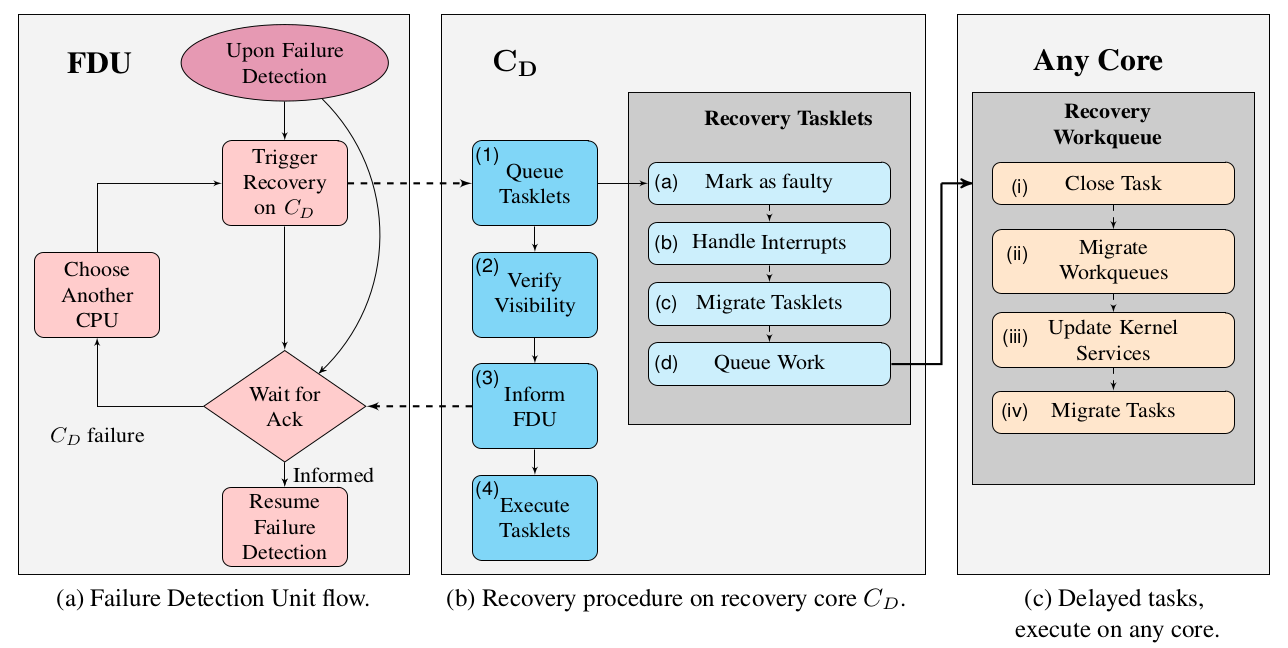
\includegraphics[width=10cm]{recovery_procedure}
	\centering
	\label{fig:migration}
\end{figure}


To enable recovery, the remaining system needs to notice the crash of one of the cores. For this, the paper requires a failure detection unit (FDU), which can either be implemented in hardware or software and reliably detects failures of one or more cores in the system. This FDU will trigger a migration procedure as described in figure \ref{fig:migration}, migrating all tasks to another core. For this, one core will be chosen to carry out the migration procedure, this will preferably be a core on another die to minimize the risk of cascading failures hitting the recovery procedure. %optional: The tasklets are equipped with IDs to overcome the possibility of multi-execution in case a cascading failure of the rescuing core.
This procedure involves the following steps, of which some are executed in high priority kernel tasklets\footnote{Kernel tasklets are small pieces of kernel work that need to be handeled in a very timely manner, usually before the next scheduling context switch} on the rescuing core and some scheduled into the global run queue and executed later on any core. On an abstract level, the task summarized are
\begin{enumerate}
	\item \textbf{Handle time-critical tasks} The failing core must be marked faulty inside the kernel as early as possible, so no further work is scheduled to this core and no further interrupts are sent here. Also time-critical tasks that were assigned to the failing core need to be migrated as soon as possible - tasklets are reassigned and spurious\footnote{Spurious interrupts are interrupts that are triggered without the underlying cause, usually they are physically induced or triggered by soft-errors} interrupts of all types will be sent to cope for potential hardware interrupts this core could have held.
	\item \textbf{Notify FDU} The first point of work needs to be executed as fast as possible, and in case of a cascading failure of the core doing the rescue work, the FDU will have to restart the recovery procedure on another core. Thus the FDU needs notification about the successful execution of the timecritical recovery parts, everything else is assigned to the global run queue and will be executed by any core at a later point in time.
	\item \textbf{Migrate work} The work which was assigned to the failing core, such as processes and threads which executed on that core should not stall forever. The process which was executing at the time of the failure will be terminated, as the registers and thus a significant part of the application state was lost. All other assigned work items will be reassigned to core 0 (the OS loadbalancer will rebalance that work later on) and depending on the operating system some services might need updates.
\end{enumerate}

This approach already seemed solid against userspace and idle failures, however if the core should fail while it holds a kernel lock, this lock will never be released and another core might deadlock. To overcome this, the team offered a solution to use lock-elision\footnote{Lock-elision assumes critical sections to be uncritically, executing them without a lock and rolling back upon detection of an actual conflict} supported by HTM, making it unnecessary for the kernel to still hold locks in almost all cases and less critical for the code to abort in that section. They only implemented this feature as a case-study, covering only run-queue locks.

\section{Evaluation}

They did two evaluations, one in a large scale context on virtual machines and one on a physical machine. Also they evaluate the performance impact by introducing HTM lock-elision. 

On the virtual machine, they applied typical workloads by using benchmarks and workloads in a normal server context. They modified the QEMU virtual machine to terminate a single random core at a random time when it is either in user mode, kernel mode or in idle. They ran these tests with the HTM transaction feature disabled and repeated these experiments to improve statistical significance. Even though operating with disabled transactions, the solution was able to survive all userspace and idle failures and 70\% of the kernel failures. They evaluated where in the kernel these crashes happened and found that all crashes happened in passages where the code held some kind of lock.

\begin{figure}[t]
	\caption{A typical recovery timeline}
	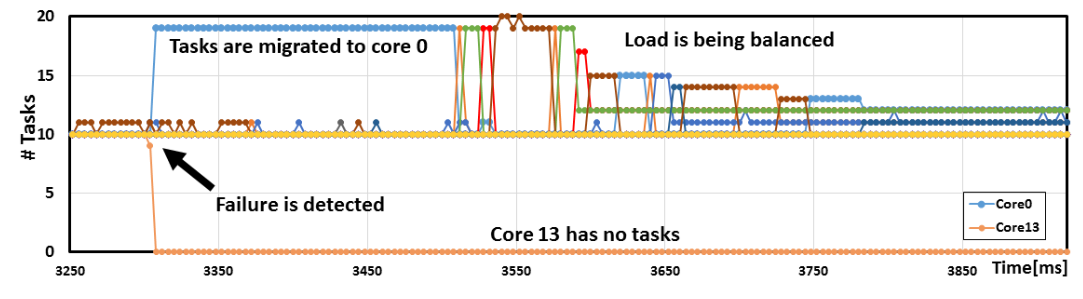
\includegraphics[width=10cm]{timeline}
	\centering
	\label{fig:timeline}
\end{figure}


They also checked if their approach to migrate all tasks to the first free core would include a significant misbalance, however as displayed in figure \ref{fig:timeline}, they concluded that the typical linux scheduler is well able to rebalance an unbalanced system over the time.

On the physical system, they emulated a crashing core by placing a endless loop inside a non-preemtive context at 100 representative kernel functions, causing the core executing that code snippet to not respond anymore. At first they ran this experiment multiple times with a normal linux installation and found it freezing every time after a few seconds. They repeated this experiment with the HTM-enabled CSR solution and found the system recovering in all cases. To display the effects on the running processes, they demonstrate CSR using a server running virtual machines. Only those virtual machine executed on the failing core was terminated, the other machines continued execution.

At last, they evaluated the performance impact of using lock-elision with HTM in comparison to a normal kernel. They found their modified kernel to be more energy efficient and performant, beneath bringing the additional failure security in the CSR context.

\section{Discussion}

This paper offers the first approach for an operating system to survive in the presence of core failures, thus we will not be able to compare this paper against existing or previous approaches. It is a clear benefit to the reliabiliy of any operating system, and the overhead of holding some additional kernel bitmaps and a bigger kernel code is negligible in contrast to the advantages.
Still there are some points which lower the overall usefulness of the paper or can be critizised. Also there are some weaknesses which are already adressed within the paper
\begin{itemize}
	\item A lot of operating system structures are assuming code to be executed (locks, interrupts)
	\item All load is migrated to core 0, which results in a temporary high-load situation of that core
\end{itemize}

We will not discuss the weaknesses that are already ruled out in the paper itself, as we regard the discussions of these points in the paper as very complete. However, we have our own points of critics about the paper, which we will address in the following subsections.

\subsection{HTM required to rollback}
To cover for kernel failures, Shalev et al. used HTM transactions to wrap all kernel locks. The approach has the requirement that upon a processor fail within a HTM transaction, the HTM implementation will rollback the transaction and thus release the lock. Combined with the concerns expressed in section \ref{cachefailure}, we doubt every implementation is actually able to provide that promise, especially in a real world scenario. Intel TSX, a HTM implementation by Intel, is a feature of the CPU chip and thus all the functionality is located close to potentially failing CPU cores, and the implementation itself might be affected by physical core destruction. We did however not find any literature to prove or disprove them.

%TODO research actual HTM specification for hardware failures
\subsection{FDU} \label{fdu}
One fundamental requirement of the work is a working failure detection unit, that can reliably detect if a core has failed and that will not stop working itself. However, in the paper there was very little discussion about the properties of this unit, except for saying that it can be implemented in hardware. This is indeed true, as there are several patents for failure detection units \cite{IBMFDU} \cite{FujitsuFDU}, however it is questionable if this unit can be assumed present on all machines. If not, this FDU would need to be emulated in software, bringing multiple drawbacks. At first, a software FDU would be bound to a process which is bound to a CPU which is assumed to be unreliable in this paper. So a solution with failover instances would need to be set up, which was not discussed in this paper. Also the FDU offers a potential vulnerability, enabling an attacker to fully disable the machine if taken over.

It is also imaginable of the FDU noticing false positives, shutting down an intact processor. In this case, the migration procedure would be triggered terminating the process that was running at that time and migrating all other processes in this CPU's execution queue to other cores. However, that CPU would still be functioning and possibly still executing tasks inside its execution queue. Thus, at that point there would be two cores executing the same program flow, the old one and the one where the process was migrated to. This will for most programs result in data-corruption or crashes, as code which was assumed to run sequential suddenly runs with two parallel instances accessing the same memory locations.

\subsection{Failures in Kernelspace}
Through wrapping kernel operations, the paper never reached 100\% failure tolerance on their given model. There were some code parts which could not be covered inside transactions, for example the context-switch which requires a TLB flush and thus can not be protected by HTM. Also, on the other locks they had the fallback path of using the code unprotectedly after 10000 failed retries, which makes it possible for the kernel to be in the fallback path during failure. Though it was never explicitely stated that reaching 100\% of coverage was an aim and generally is very untypical for the research area of fault-tolerance, they put quite a lot of effort in reaching that aim.

The approach by the paper requires HTM to be present to tolerate kernel failures. However, HTM is a very new and untested %TODO cite bugs in haswell and skylake?
feature. It is present in only some modern CPUs and thus this feature addresses only a small audience. However the paper title assumes it should be addressed to commodity software. It was not discussed if the approach would also work with Software Transactional Memory. However, as hardware transactional memory is on the rise, it could be a widely available feature soon, so we don't regard this as problematic.

Furthermore they only implemented their feature for run-queue locks, making up only a fraction of all kernel lock structures. They hinted at TxLinux \cite{TxLinux}, a linux kernel implementation successfully replacing all locks with transaction, to be a proof of feasibility of this approach. We do not know why they did not use TxLinux in the first place already and instead replicated a part of the TxLinux work in their paper. Both papers strived for high transaction coverage, and it would have been less work with higher effect to just use what is there already. Also, the paper does not state problems with cornercases as TxLinux does, which could either be due to their partial implementation not being representative enough or doing something else than TxLinux or due to them not checking careful enough. All this was not discussed in the paper and we can just assume.

The CSR approach is also usable without the kernel transaction feature, empirically measured securing 70\% of all kernel failures and all userspace failures already while imposing very little overhead. The modifications necessary to only tolerate userspace-failures are far smaller making them more easy to review for security or functionality implications on other code, which makes me more optimistic that a future linux update will incorporate this feature. The paper stated their solution offers the possibility to disable kernel transactions, still making an impact on the total availability.

\subsection{Statistical implications of hardware failures}
There is quite some research on the statistics of hardware failures. An empirical analysis of one million consumer PCs \cite{Microsoftfailures} reveals that as soon as one physical hardware failure occurs, the machine is a lot more likely to experience another failure within a short timespan. Just for CPU-system failures, the prior probability of a failure increases by factor 100 once the machine failed once. Another paper \cite{HPCfailures} speaks of factor 5-20 regarding all kind of single node failures. 

These statistics have not been regarded in the paper. They pose the question if the effort to save a node or CPU as soon as they failed once should be taken, or if in a server context a once failing component should be abandoned for the future, as it is likely to fail again. Thus, if this method is used in a server context, it would only be helpful in the very moment the core fails, as any longterm usage of a partially failing node is not recommendable. For this short-term moment the mechanism holds an availability advantage, as only one process need to be restarted at a time, however no longterm measures such as migrating work to another node \cite{VMLiveMigration} were discussed. 

\subsection{Cascading failures}
In the paper it was already mentioned that cascading failures are likely to occur. Though these assumption was not based on statistics, they make sense as some failure reasons such as overheating will happen to the whole chip. To overcome the problems of that, the algorithm was optimized and analyzed to allow another failure to happen even during the migration process and cores from another die are chosen with preference to perform the migration work. However, no preventive measures were implemented or discussed. Maybe it would be a good idea to modify the loadbalancer to temporarily reduce the load on a chip which just had a failure, as it could decrease the amount of potential processes shutdown in case of another failure. If there is only one chip, this is of course not possible. Also, it would have been possible to link to research in cluster reliability here and suggest to already decrease the load on the node in that cluster, if it is used as a server.

\subsection{Component limitations and failure model} \label{cachefailure}
Shalev et al. described a very specific failure model, which they wanted to tolerate. However the scope of this failure model is quite small, making it possibly less useful for real world applications. At first, they limit to CPU failures. Though being the executing unit in every computer, failures can also happen at many other places. However, it would have exceeded the scope of this paper to handle DRAM, bus, storage and other failures aswell and there are technologies to partially cope with those already.

Furthermore they limit possible failures to the actual executing units only, requiring the cache to stay intact despite being on the same chip. Their reference to real-world applications was the case of a failed transistor, which makes the whole core unable to function correctly, but they did not discuss transistors which are part of the cache. Although it was difficult to find specific literature on the probability of a cache failure, cache is taking a high portion of transistors on modern chips and ignoring the chance of it failing seems like ignoring a big part of the problem. We are unsure if it would have been effectively possible to allow for cache failures, as most of the modern HTM implementations rely on cache mechanisms and even without HTM usage any data could get lost, corrupting the state of arbitrary applications. However, there was no discussion of this limitation at all.

Another issue with their failure model is the assumption that a faulty core will not get back online again. This might be the case if the core actually burned out, but it is imaginable that a temporary bus-disconnect or a soft-error caused the core to just fail temporarily. This point of critics is related to a false positive by the FDU as discussed in Section \ref{fdu} and could aswell lead to data corruption or crashes if the core comes back online and continues executing its previous instruction pipeline. There is no work done to prevent this nor was this issue discussed in the paper.

\subsection{Means of testing}
The testing never involved a real world scenario of a failing core, they never physically destroyed a core and tried to recover from that. The testing scenarios included a QEMU VM environment, where they randomly terminated a cpu thread to simulate the failure of a core and an example on a machine, where they simulated a failing core by invoking an endless loop in a non-preemtive\footnote{Non-preemtive means execution can not be interrupted from outside, disabling all scheduling mechanisms} kernel context. Both scenarios were tailored to fit their assumed failure model, but none was truly realistic - it would have been better to install this operating system on a bigger multinode cluster and wait for one node actually failing the assumed way. However we see the obvious cost problem and assume this as outside the budget and not actually a flaw of the research work.

Also they did not go very much in detail about their cascading failure testing. On the physical machine, they did one experiment, crashing the rescuing core before sending the ack to the FDU and the test went as expected. We think it might have been good to execute this test several times with different delays between the cascading failures, also trying to crash other cores than the nominiated rescuing core.

At last, they did not name a number of repetitions/measurements for any of their tests, making it impossible to judge the significance of their test results.

%\subsection{No perfect protection}

%The given approach requires other means of fault-tolerance to be in place already, as the shutdown of the process currently active on the core can not be avoided. It is already mentioned that this approach can only be used with other means in place, and checkpointing is given as an example. So in the given model, each process can already tolerate spontaneous shutdown. To reduce the chances of failure for each process undeniably increases it's availability, however there is no effect on the tradeoff to consistency or latency as failure chances are still far from zero. This was never an aim of this approach, and there is a lot of research available concerning the tradeoffs between these and how to manage fault-tolerance on a more abstract level. The CSR approach makes none of these approaches obsolete and does not aim to do so. It is of undeniable but not of groundbreaking impact by reducing the chance of a full node failure, not by making it impossible.

\section{Conclusion}

We think the paper itself is an enrichment, as this mechanism offers a benefit in availability to any computer system combined with a low overhead. However, the writers did not see the work in a real-world application, trying to reach 100\% failure tolerance within their given failure model. We would have preferred if the focus was rather to incorporate Cache-failures as well or trying to integrate it into a multi-cluster approach, for example by linking to existing approaches to migrate all remaining virtual machines on the node upon the first detected failure to another node. These approaches could potentially have benefitted to the total availability improvement in a real world scenario, but were not discussed in favor of a very in-depth view of this mechanism.

At the state the work is right now, we would not recommend to incorporate the kernel-transaction approach into the commodity linux kernel, however we think the solution without transactions is a great candidate for a future linux release. We would recommend to the authors put some effort into incorporating the TxLinux approach, as this would open the possibility to cover wide areas of the kernel with transactions, reaching better failure tolerance and also making the system benefit from the other advantages of hardware lock-elision. 

\bibliographystyle{plain}
\bibliography{handin} 

\end{document}
